% CVPR 2027 submission, version 2.0 (2026-10-13). Refocused on the teaching round (restricted teacher, competing students).
% v1 (audit-first) kept as main_v1_3_pre_refocus.tex. Audit details for DeepEyes / SlideChat / VLM zoom moved to supp.tex.
\documentclass[10pt,twocolumn,letterpaper]{article}
\usepackage[review]{cvpr}
\usepackage{graphicx,booktabs,amsmath,amssymb,multirow,xcolor}
\usepackage{cuted,caption}
\definecolor{cvprblue}{rgb}{0.21,0.49,0.74}
\usepackage[pagebackref,breaklinks,colorlinks,allcolors=cvprblue]{hyperref}
\newcommand{\pend}[1]{{\color{red}[#1]}}
\def\paperID{*****}\def\confName{CVPR}\def\confYear{2027}
\title{The Teaching Round: Deciding Gigapixel Slides from a Few Patches\\Presented by Readers That Cannot Be Trusted}
\author{Anonymous}
\begin{document}
\maketitle

\begin{abstract}
Gigapixel pathology slides and high-resolution images are rarely decided from the whole input: a selector picks a few regions and a judge decides from them. We first show that this interface is the weak point. With slide, features and judge fixed, choosing different \emph{authentic} patches drives attention top-$B$ MIL on CAMELYON16 from 0.97 to 0.00 balanced accuracy, non-adversarial alternative selectors already change 9--61\% of BCNB decisions, and one adversarial crop breaks 38--57\% of correct VLM answers on V* and HR-Bench. We then study a remedy modelled on the clinical teaching round. Two students read the whole slide and are assigned opposite diagnoses, so one of them is always a devil's advocate; a teacher that never looks at the slide itself decides from the patches the students present. On CAMELYON16, a teacher that sees 2 of $\sim$9{,}700 patches reaches 0.94 balanced accuracy (full-slide MIL: 0.98), stays at 0.90--0.98 from a single tumor patch to 20\% tumor against greedy and look-ahead devil's advocates, and keeps 0.92 with a second encoder on which full-slide MIL is unstable. Because only the presented patches must be read well, cheap ResNet50 students presenting to a UNI teacher reach 0.96 balanced accuracy, within two points of full-slide UNI MIL, at 1/15 of the encoder FLOPs (1/5 of the A100 time). Matched-budget controls locate the effect: one-shot class-conditioned counter-selection works as well as alternating debate, whereas two cooperative readers collapse when one is compromised, and the teacher's own uncertainty cannot replace the opposing student, because omitted evidence leaves it confidently wrong. Letting the teacher ask follow-up questions adds nothing when both students are competent; when the honest student is unreliable, a learned questioning policy spends more patches on contested slides and beats a silent teacher at matched average budget, whereas questions triggered by the teacher's own confidence are no better than random extra patches. The protocol needs a competent honest reader and helps where single witnesses decide; on diffusely expressed labels (BCNB receptor status) it does not beat random sampling. A label-free variant with one advocate per answer option carries over to VLMs.
\end{abstract}

%=====================================================================
\section{Introduction}\label{sec:intro}
A whole-slide image has $10^4$--$10^5$ patches; a 4K photograph has more detail than a vision-language model reads at once. Practical systems therefore \emph{select}: attention MIL keeps the top-scored patches~\cite{ilse2018abmil}, retrieval picks question-relevant regions~\cite{beacon2026}, and zoom agents answer from the crops they request~\cite{wu2024vstar,zheng2025deepeyes}. The judge that decides is accurate only if the selector shows it the right evidence, and nothing in the pipeline checks that.

We first measure how much the choice of evidence alone controls the decision (Sec.~\ref{sec:audit}), following the paired protocol of BagShift~\cite{bagshift2026}: slide, features and judge fixed, only the selected authentic regions change, at a fixed inspection budget $B$. A selector that hides the lesion, or that adds authentic normal tissue around it, flips almost every CAMELYON16 decision; selectors that a different but reasonable pipeline would use already disagree with the deployed one on up to 61\% of BCNB slides and lower its accuracy.

The main question of the paper is how a judge that can read only $B$ items should be protected when the readers who choose them cannot be trusted. We borrow the answer from medical education. In a teaching round, students who have studied the case present findings for competing diagnoses, one of them deliberately as a devil's advocate, and a senior physician questions them and decides. The senior does not re-read the case: otherwise the students would be unnecessary. We implement exactly this division of labour. \emph{Students} read the whole slide and each argues an assigned label with authentic patches; the \emph{teacher} sees only what they present and decides (Fig.~\ref{fig:qual}). We study two teachers: one that cannot ask questions, and one that can ask follow-ups (``show me more'', ``show me what surrounds that patch'') when it is unsure.

\paragraph{Contributions.}
\begin{itemize}
\item \textbf{The teaching round as a restricted-judge protocol} with an explicit inspection budget, devil's-advocate threat model and on-policy teachers, evaluated against attention top-$B$, cooperative queriers, single consultants, random masking and full-slide MIL at matched budget (Sec.~\ref{sec:setup}, \ref{sec:results}).
\item \textbf{Where the robustness comes from.} Controls show that class-conditioned counter-selection, not interaction or presenter identity, is the effective ingredient; that the teacher's own doubt cannot replace the opposing student; and, on a fixed-judge sparsity grid, that the protocol tracks the \emph{number} of tumor witnesses while random masking tracks the probability of sampling one.
\item \textbf{Cheap students, expensive teacher.} Students that read the slide with a cheap encoder and present to a teacher that encodes only the presented patches come within two points of full-slide MIL at 1/15 of the encoder FLOPs (1/5 of the A100 time).
\item \textbf{Questions.} A teacher that asks follow-up questions, with fixed and learned questioning policies, compared with a silent teacher at equal inspected patches across honest-student strength: questions help only when the honest student is unreliable, and only when learned from the state of the round rather than triggered by the teacher's confidence.
\item \textbf{A short selection audit} that motivates the problem: omission and override in MIL, natural-selector disagreement, steerable VLM zoom, and models whose apparent robustness comes from ignoring the selected evidence (DeepEyes, SlideChat; details in the supplement).
\end{itemize}
We do not claim worst-case soundness. The students read every patch, but they need not read it well: with ResNet50 students and a UNI teacher that encodes only the presented patches, the teaching round comes within two points of full-slide UNI MIL at 1/15 of the encoder FLOPs and 1/5 of the A100 encoder time (Sec.~\ref{sec:results}).

%=====================================================================
\section{Related work}\label{sec:related}
\paragraph{Evidence selection in MIL and zoom agents.} BagShift~\cite{bagshift2026} introduced the paired protocol of changing only the patch selector for a fixed slide, features and predictor, for deployment selectors on CAMELYON16 and PANDA; we use it as our audit and add adversarial, transferred and hypothesis-conditioned selectors and witness analysis. Pixel-level attacks on MIL~\cite{mil_adv2022,foote2021now} perturb inputs rather than selection. Sufficiency methods (FOCI, GCE-MIL, ReaMIL, CAR-MIL)~\cite{foci2026,gcemil2026,reamil2026,carmil2026} ask which subsets suffice, and BEACON~\cite{beacon2026} acquires evidence by expected information gain; all assume a cooperative selector. V*~\cite{wu2024vstar}, ViCrop~\cite{zhang2025vicrop}, DeepEyes~\cite{zheng2025deepeyes} and Mini-o3~\cite{minio3} answer from zoomed crops, and MED~\cite{med2026} separates tool-induced from intrinsic gains; our crop substitutions are a complementary causal test (supplement).
\paragraph{Debate and prover--verifier games.} Irving et al.~\cite{irving2018debate} proposed debate with a sparse-pixel judge and discuss gigapixel inputs. Merlin-Arthur classifiers~\cite{waldchen2024merlin} and the Neural Concept Verifier~\cite{ncv2026} analyse helpful and misleading provers for a feature verifier; prover--verifier games~\cite{anil2021pvg,kirchner2024pvg,hammond2025nip} and LLM debate~\cite{khan2024debate,kenton2024scalable} study text, and visual debate has been studied with text-only judges~\cite{adhikari2025debating} and for deception~\cite{fang2026debateimages}. A public report found image-cell debate close to a random-mask ensemble~\cite{quantilized_debate}. We do not propose a new debate game; we ask when a budget-restricted visual judge needs one, which of its ingredients matter, and whether questioning the students helps.

%=====================================================================
\section{Setup}\label{sec:setup}
\paragraph{Restricted teacher.} An input is a set of items $x=\{x_i\}_{i=1}^N$ (patch features, or image tiles). A teacher $J$ decides from a presented set $S\subseteq[N]$ with $|S|\le B$, the \textbf{inspection budget}. Every comparison is at equal $B$; in two-student protocols each student presents $B/2$ items.
\paragraph{Students and threat model.} Students see all items. Each is assigned a label and presents the items that most support it, greedily on the teacher's exact incremental output given what has been presented so far (white-box), or with a look-ahead rollout. Whichever student is assigned the wrong label is the \emph{devil's advocate}; it uses authentic items only. The teacher sees each item with a presenter flag (which label its student argues), never the truth. Baselines at the same $B$: the judge's own attention top-$B$ (deployed), a V-IP querier~\cite{chattopadhyay2023vip}, a single consultant arguing an assigned label, two independent cooperative readers, uniform random masking (one draw, or 32 draws averaged), and full-slide MIL as an unrestricted reference.
\paragraph{Teacher without questions (A).} Both students present until $B$ items are shown; the teacher decides once. Variants: alternating debate~\cite{irving2018debate}; static counter-selection (each student chooses all its items without seeing the other's); static without flags.
\paragraph{Teacher with follow-up questions (B).} The round opens with one item per student. While the teacher's confidence $\sigma(|\ell|)$ is below $\tau$ (or as a learned policy decides), it asks one of: \emph{trail}: the student it currently disagrees with presents its next item; \emph{both}: both present their next item; \emph{context}: the teacher points at the leading student's most-attended item and both students must present a spatial neighbour of it (8-neighbourhood) of their choice, as a senior asks to see the surrounding tissue of a suspicious focus. A \emph{random} control adds two random items instead. The \emph{learned} questioning policy chooses among stop/trail/both/context from label-free features of the teacher state (confidence, attention entropy and mass per side, items per side, last change), trained by regressing each question's one-step gain in $\log p(\text{truth})$ on held-out training slides, with a per-item cost $\lambda$. All teachers are capped at 16 items.
\paragraph{Teachers are trained on-policy.} The teacher is a gated ABMIL~\cite{ilse2018abmil} over presented items with a presenter-flag input. It is warm-started on attention-selected and random subsets with random flags, then trained for 3--4 rounds on transcripts produced by the students against the current teacher (for B: random question sequences, all prefixes). Every baseline judge gets the same treatment. The questioning policy uses slides the teacher was not trained on.
\paragraph{Data.} CAMELYON16~\cite{c16}: 512px level-0 patches, official 270/129 split (49 tumor test slides), patch-level lesion labels, UNI~\cite{uni} features and, as a second encoder, ResNet50 Barlow-Twins features (pathology-pretrained weights of Kang et al.~\cite{kang2023benchmarking}, as distributed with torchmil). BCNB~\cite{bcnb} ER/PR/Grade-3 with CONCH~\cite{conch} features, 5-fold CV. V*-Bench~\cite{wu2024vstar} (191) and HR-Bench-4K~\cite{hrbench} (200) with Qwen2.5-VL-7B~\cite{qwen25vl} and Qwen3-VL-8B~\cite{qwen3vl}. MIL results: balanced accuracy (BA), mean$\pm$sd over 3 seeds; VQA: 95\% bootstrap CIs.

%=====================================================================
\section{The selection interface decides}\label{sec:audit}
\begin{table}[t]\centering\small
\caption{\textbf{Who chooses the patches decides} (CAMELYON16, BA, 3 seeds; full-slide ABMIL .969). Attacked = a white-box selector picks the $B$ items for the wrong label. Cons.\ = one consultant arguing an assigned label.}\label{tab:c16}
\setlength{\tabcolsep}{3pt}
\resizebox{\linewidth}{!}{\begin{tabular}{@{}lcccccc@{}}\toprule
$B$ & attn & attn (att.) & V-IP (att.) & cons.\ (att.) & rand-mask$^\ast$ & teaching round\\\midrule
2  & .974 & .021 & .000 & .000 & .556 & \textbf{.943}$\pm$.023\\
4  & .978 & .000 & .000 & .000 & .628 & \textbf{.949}$\pm$.010\\
8  & .984 & .000 & .000 & .000 & .628 & \textbf{.971}$\pm$.011\\
16 & .978 & .000 & .000 & .000 & .703 & \textbf{.958}$\pm$.008\\\bottomrule
\end{tabular}}\\[1pt]{\footnotesize $^\ast$32 random draws of $B$ items, mean logit.}
\end{table}

\begin{table}[t]\centering\small
\caption{\textbf{Plausible selectors already change decisions, and lower accuracy} (BCNB-ER, ABMIL top-$B$ judge, $B{=}8$). Flip: fraction of slides whose decision differs from the deployed selector's.}\label{tab:natural}
\begin{tabular}{@{}lcc@{}}\toprule
selector & BA & flip\\\midrule
own attention top-$B$ (deployed) & .758 & --\\
independent model's attention & .741 & .091\\
k-means coverage & .635 & .266\\
question-relevance retrieval & .613 & .177\\
confirm majority hypothesis & .525 & .232\\
confirm minority hypothesis & .581 & .608\\\midrule
black-box transfer (full-slide surrogate) & .240 & .642\\
transfer from TransMIL surrogate & .110 & .681\\
white-box greedy & .020 & .784\\\bottomrule
\end{tabular}\end{table}

\paragraph{MIL.} With slide, features and judge fixed, a white-box selector drives attention top-$B$, a V-IP querier and a single consultant to $\approx$0 on CAMELYON16 at every budget (Tab.~\ref{tab:c16}). This is a worst case; Tab.~\ref{tab:natural} separates it from deployment. Selectors that a different pipeline could plausibly use (another model's attention, coverage sampling, retrieval, hypothesis-confirming search) change 9--61\% of BCNB-ER decisions and lower BA from .758 to .525--.741, so the changed decisions are mostly worse, not just different. Attacks optimized against an independent surrogate transfer (.110--.240).
\paragraph{Omission and override.} On tumor slides, 98--100\% of successful attacks on attention top-$B$ contain no tumor patch: the dominant failure is \emph{omission}. Forcing the most-attended true witness into the selection does not protect the judge: authentic normal patches in the remaining slots still flip 99\% ($B{=}2$), 89\% ($B{=}4$) and 55$\pm$38\% ($B{=}8$) of tumor slides (\emph{override}).
\paragraph{VLMs.} For Qwen2.5-VL and Qwen3-VL on V* and HR-Bench, the model's own zoom repairs 36--68\% of wrong answers and breaks 6--8\% of correct ones, but one adversarially chosen authentic tile shown with the global view breaks 38--57\%. Two systems are insensitive to selection because they ignore it: DeepEyes~\cite{zheng2025deepeyes} calls its zoom tool on every V* question, yet substituting the ground-truth, random or adversarial crop changes at most 3\% of its answers; SlideChat~\cite{slidechat} reproduces its reported SlideBench-BCNB accuracy, but at the majority-class rate, and gives the same answers with no slide or another patient's slide (supplement). A teacher must use the evidence to be steerable, and to be protectable.

%=====================================================================
\section{The teaching round}\label{sec:results}
\begin{figure*}[t]\centering
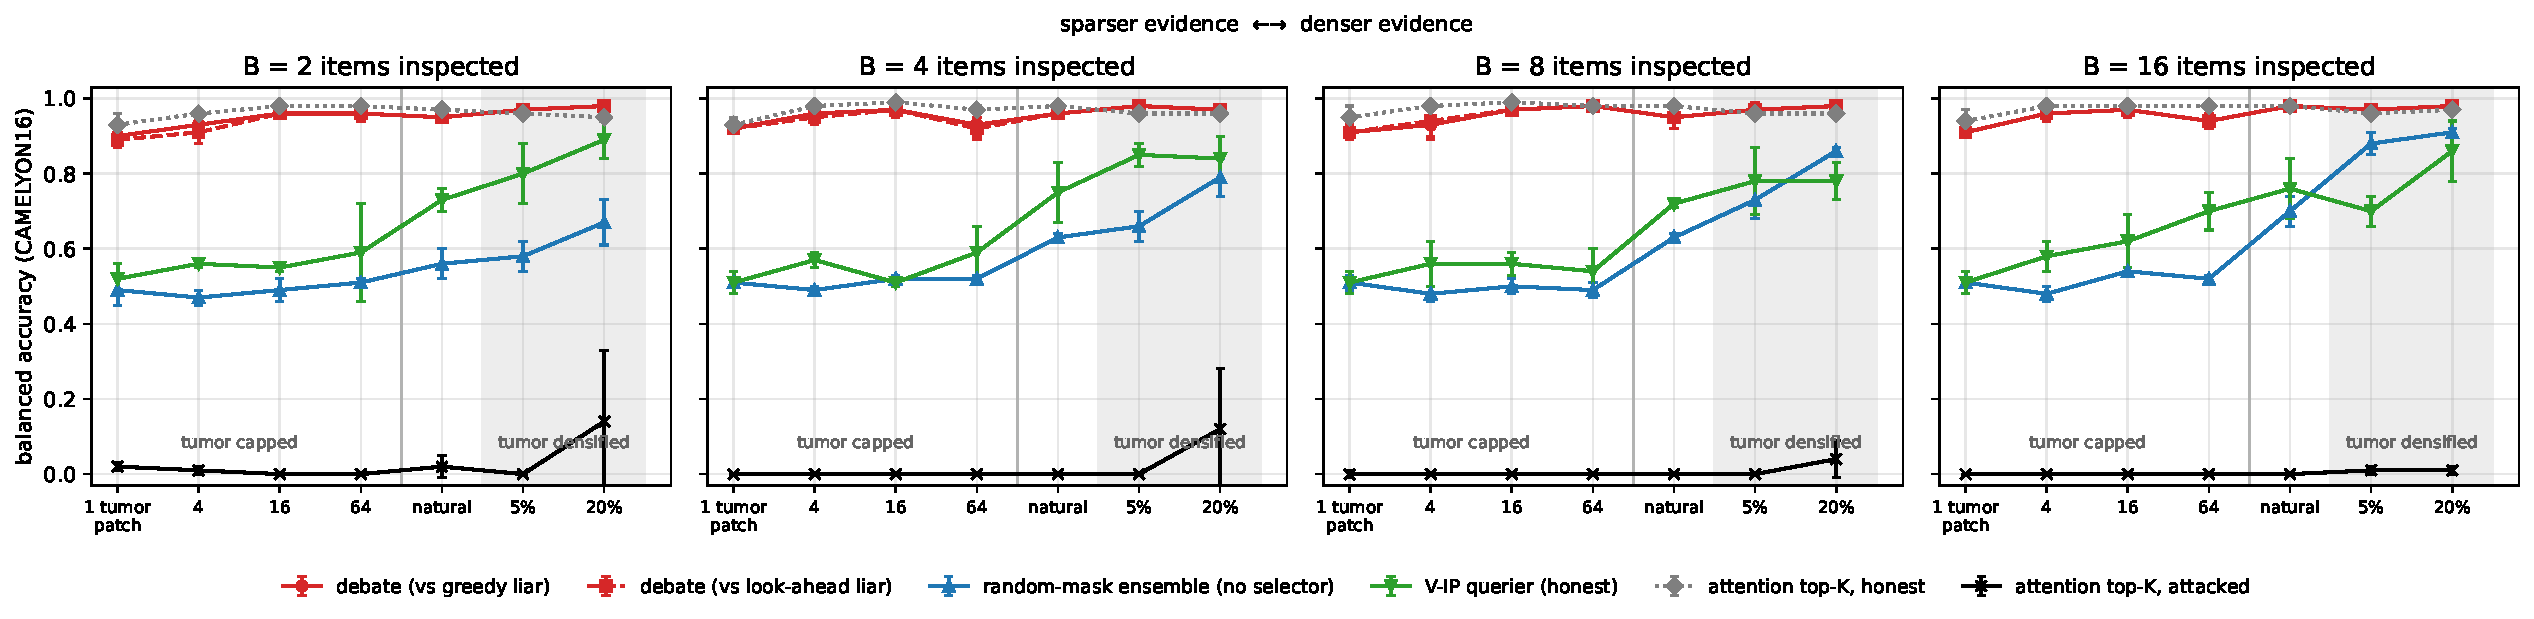
\includegraphics[width=\linewidth]{figs/fig_sparsity.pdf}
\caption{\textbf{Accuracy vs.\ evidence sparsity} (CAMELYON16, 3 seeds; judges retrained per regime; panel title = budget $B$). Left: tumor capped to 1--64 patches (other tumor patches and their neighbours dropped); right: tumor densified to 5\%/20\%. The teaching round (red) stays at .90--.98 against greedy and look-ahead devil's advocates; random masking (blue) is accurate only when evidence is dense; cooperative selectors (grey, green) collapse under attack (black).}\label{fig:sparsity}
\end{figure*}

\paragraph{A teacher that reads two patches.} The silent teacher (A) is within 1--3 points of full-slide MIL at every budget while any single selector is driven to zero (Tab.~\ref{tab:c16}). With UNI features, a teacher shown one patch from each student reaches .942$\pm$.023 BA from 2 of on average 9{,}700 patches (full slide: .978$\pm$.003); more presented patches do not help (16 patches: .928). With ResNet50 features (Tab.~\ref{tab:r50}) the teacher keeps .91--.95 at every budget while attention top-$B$ under attack falls to .09--.30, and full-slide ABMIL is unstable across seeds (.93/.50/.53), whereas teachers trained on presented items stay within .82--.97 on every seed. Across sparsity regimes (Fig.~\ref{fig:sparsity}) the teaching round is the only protocol that is both accurate and robust: at $B{=}16$ random masking rises from .51 (one tumor patch) to .91 (20\% tumor), while the teaching round stays at .91--.98.

\paragraph{Cheap students, expensive teacher.} The students only have to find candidates for each label; the teacher only has to read a few patches well. We therefore let the students read the slide with a cheap encoder (ResNet50 Barlow-Twins) and encode only the presented patches with UNI for the teacher (Tab.~\ref{tab:cheap}, Fig.~\ref{fig:cheap}). Per slide this costs $N$ ResNet50 passes plus $B$ UNI passes instead of $N$ UNI passes, 15$\times$ fewer encoder FLOPs and 5.3$\times$ less A100 encoder time (8.6\,s vs.\ 1.6\,s per slide; fp16, batch 256). Over 6 seeds, ResNet50 students with a UNI teacher reach .937$\pm$.021 at $B{=}2$ and .958$\pm$.015 at $B{=}8$, within 2 points of full-slide UNI ABMIL (.975$\pm$.010) and on par with UNI students (.93--.96); a look-ahead devil's advocate does not lower it (.927--.958), and blank patches give .500. The cheap encoder alone is not enough: full-slide ResNet50 ABMIL is unstable (.54--.92 across seeds) and ResNet50 students with a ResNet50 teacher stay at .90--.92. Published MIL methods on the same full-slide UNI features reach .91--.95 BA (.92--.96 with a validation-tuned threshold; AUC .975--.991) at 8.6\,s per slide, and on full-slide ResNet50 features .67--.91 at the same 1.6\,s as ours (Tab.~\ref{tab:published}): the teaching round matches the best full-slide UNI methods at the cost of full-slide ResNet50 methods. The cheap reader is good enough to \emph{find} witnesses, and the expensive encoder is needed only to \emph{read} the few it presents. A cascade without students, in which full-slide R50 ABMIL selects its top-$B$ patches for a UNI judge, costs the same and reaches .94--.99 on the five seeds where R50 ABMIL trains well, but inherits its failure on the sixth (.42--.56) and falls to .40--.55 when the selector is compromised; the teaching round stays at $\ge$.90 on every seed and against the devil's advocate. Students need not read every patch either: reading a stride-2 subgrid and then the neighbourhoods of each student's best candidates (28\% of patches, 0.46\,s, 18$\times$ faster than full-slide UNI) keeps .931$\pm$.022 at $B{=}8$ (.928 with a look-ahead devil's advocate), above UNI ABMIL on a uniform subgrid of similar cost (1/16 grid, 0.54\,s: .892$\pm$.016); reading 6--17\% drops to .84--.89 (Fig.~\ref{fig:cheap}).

\begin{table}[t]\centering\small
\caption{\textbf{Cheap students, expensive teacher} (CAMELYON16, BA mean$\pm$sd, 6 seeds). Students$\to$teacher encoders; only the $B$ presented patches are encoded for the teacher. DA = look-ahead devil's advocate. Cascade: full-slide R50 ABMIL selects its top-$B$ attended patches, a UNI judge decides; attacked = the selector picks patches for the wrong label. Encoder cost per slide ($\sim$9{,}700 patches, A100, fp16): full-slide UNI 1194 TFLOPs / 8.6\,s; R50 students + $B$ UNI patches 79 TFLOPs / 1.6\,s. Full-slide ABMIL: UNI .975$\pm$.010, R50 .836$\pm$.133 (.54--.92).}\label{tab:cheap}
\setlength{\tabcolsep}{2.5pt}
\resizebox{\linewidth}{!}{\begin{tabular}{@{}lcccccc@{}}\toprule
 & & \multicolumn{3}{c}{teaching round} & \multicolumn{2}{c}{cascade (no students)}\\\cmidrule(lr){3-5}\cmidrule(l){6-7}
$B$ & random$\to$UNI & UNI$\to$UNI & \textbf{R50$\to$UNI} & R50$\to$UNI, DA & R50 top-$B\to$UNI & attacked\\\midrule
2 & .549{\tiny$\pm$.063} & .929{\tiny$\pm$.017} & \textbf{.937}{\tiny$\pm$.021} & .927{\tiny$\pm$.023} & .879{\tiny$\pm$.182} & .476{\tiny$\pm$.039}\\
4 & .547{\tiny$\pm$.032} & .950{\tiny$\pm$.021} & \textbf{.941}{\tiny$\pm$.026} & .947{\tiny$\pm$.023} & .899{\tiny$\pm$.153} & .472{\tiny$\pm$.046}\\
8 & .581{\tiny$\pm$.026} & .952{\tiny$\pm$.025} & \textbf{.958}{\tiny$\pm$.015} & .958{\tiny$\pm$.017} & .887{\tiny$\pm$.192} & .490{\tiny$\pm$.029}\\
16 & .637{\tiny$\pm$.025} & .962{\tiny$\pm$.019} & \textbf{.952}{\tiny$\pm$.029} & .949{\tiny$\pm$.030} & .883{\tiny$\pm$.207} & .503{\tiny$\pm$.038}\\\midrule
A100 s / slide & $<$.02 & 8.6 & 1.6 & 1.6 & 1.6 & 1.6\\\bottomrule
\end{tabular}}\end{table}

\begin{table}[t]\centering\small
\caption{\textbf{Published MIL baselines} (CAMELYON16 test, $n{=}129$; reference implementations from torchmil~\cite{torchmil}, same features, split, class weighting and validation-AUC epoch selection; 3 seeds, ours 6). BA at logit 0 for all methods, and for the baselines also at the threshold maximising validation BA. Encoder time: A100, fp16, $\sim$9{,}700 patches per slide; aggregator time is per slide on an A100.}\label{tab:published}
\setlength{\tabcolsep}{2.5pt}
\resizebox{\linewidth}{!}{\begin{tabular}{@{}llccccc@{}}\toprule
method & encoder & AUC & BA & BA (val.\ thr.) & enc.\ s/slide & agg.\ ms\\\midrule
ABMIL~\cite{ilse2018abmil} & UNI & .990{\tiny$\pm$.004} & .946{\tiny$\pm$.012} & .959{\tiny$\pm$.020} & 8.6 & 0.5 \\
CLAM-SB~\cite{lu2021data} & UNI & .991{\tiny$\pm$.002} & .914{\tiny$\pm$.046} & .959{\tiny$\pm$.002} & 8.6 & 0.8 \\
DSMIL~\cite{li2021dual} & UNI & .975{\tiny$\pm$.013} & .932{\tiny$\pm$.025} & .923{\tiny$\pm$.019} & 8.6 & 0.4 \\
TransMIL~\cite{shao2021transmil} & UNI & .984{\tiny$\pm$.012} & .944{\tiny$\pm$.009} & .960{\tiny$\pm$.011} & 8.6 & 10.8 \\
DTFD-MIL~\cite{zhang2022dtfd} & UNI & .977{\tiny$\pm$.010} & .926{\tiny$\pm$.028} & .923{\tiny$\pm$.039} & 8.6 & 5.2 \\
\midrule
ABMIL~\cite{ilse2018abmil} & R50 & .940{\tiny$\pm$.006} & .910{\tiny$\pm$.018} & .867{\tiny$\pm$.048} & 1.6 & 0.8 \\
CLAM-SB~\cite{lu2021data} & R50 & .945{\tiny$\pm$.009} & .862{\tiny$\pm$.011} & .906{\tiny$\pm$.019} & 1.6 & 1.3 \\
DSMIL~\cite{li2021dual} & R50 & .945{\tiny$\pm$.015} & .874{\tiny$\pm$.048} & .892{\tiny$\pm$.008} & 1.6 & 0.6 \\
TransMIL~\cite{shao2021transmil} & R50 & .729{\tiny$\pm$.166} & .668{\tiny$\pm$.173} & .724{\tiny$\pm$.157} & 1.6 & 11.1 \\
DTFD-MIL~\cite{zhang2022dtfd} & R50 & .821{\tiny$\pm$.141} & .754{\tiny$\pm$.175} & .795{\tiny$\pm$.108} & 1.6 & 5.5 \\
\midrule
our judge, full slide & UNI & .997{\tiny$\pm$.003} & .975{\tiny$\pm$.010} & -- & 8.6 & -- \\
teaching round $B{=}2$ & R50$\to$UNI & .957{\tiny$\pm$.019} & .937{\tiny$\pm$.021} & -- & 1.6 & -- \\
teaching round $B{=}8$ & R50$\to$UNI & .971{\tiny$\pm$.014} & .958{\tiny$\pm$.015} & -- & 1.6 & -- \\
\quad + look-ahead DA & R50$\to$UNI & .969{\tiny$\pm$.011} & .958{\tiny$\pm$.017} & -- & 1.6 & -- \\\bottomrule
\end{tabular}}\end{table}

\begin{figure}[t]\centering
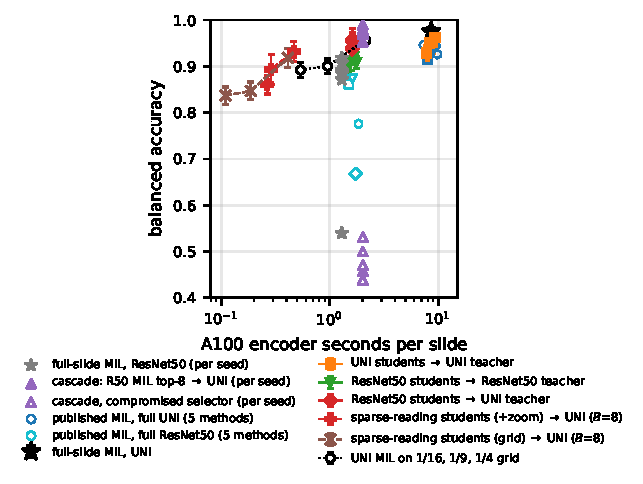
\includegraphics[width=\linewidth]{figs/fig_cheap.pdf}
\caption{\textbf{Accuracy vs.\ encoder compute} (CAMELYON16, 6 seeds, $B\in\{2,4,8,16\}$; sparse-reading points $B{=}8$). ResNet50 students presenting to a UNI teacher (red diamonds) come within two points of full-slide UNI MIL (black star) at 1/5 of the A100 encoder time; students that read only part of the slide (red crosses: subgrid + neighbourhoods of candidates; brown: subgrid only) trade accuracy for up to 18--77$\times$ speed-ups and lie above UNI MIL on uniform subgrids (open circles). A cascade with the same cost (purple, per seed) fails when its R50 selector fails or is compromised (open triangles).}\label{fig:cheap}
\end{figure}

\begin{table}[t]\centering\small
\caption{\textbf{Second encoder} (CAMELYON16, ResNet50 Barlow-Twins features; BA mean$\pm$sd, 3 seeds). Full-slide ABMIL: .93 / .50 / .53 per seed.}\label{tab:r50}
\setlength{\tabcolsep}{3pt}
\resizebox{\linewidth}{!}{\begin{tabular}{@{}lccccc@{}}\toprule
$B$ & attn & attn (att.) & cons.\ (att.) & rand-mask & teaching round\\\midrule
2  & .78{\tiny$\pm$.22} & .30{\tiny$\pm$.21} & .27{\tiny$\pm$.15} & .52{\tiny$\pm$.04} & \textbf{.92}{\tiny$\pm$.04}\\
4  & .75{\tiny$\pm$.24} & .24{\tiny$\pm$.18} & .12{\tiny$\pm$.09} & .51{\tiny$\pm$.09} & \textbf{.92}{\tiny$\pm$.02}\\
8  & .79{\tiny$\pm$.15} & .14{\tiny$\pm$.14} & .29{\tiny$\pm$.16} & .60{\tiny$\pm$.02} & \textbf{.91}{\tiny$\pm$.06}\\
16 & .79{\tiny$\pm$.14} & .09{\tiny$\pm$.07} & .45{\tiny$\pm$.03} & .64{\tiny$\pm$.07} & \textbf{.95}{\tiny$\pm$.01}\\\bottomrule
\end{tabular}}\end{table}

\begin{table}[t]\centering\small
\caption{\textbf{Which ingredient matters?} CAMELYON16 BA (mean$\pm$sd, 3 seeds), every protocol with its own on-policy judge from the same warm start, equal budget $B$.}\label{tab:mech}
\setlength{\tabcolsep}{3pt}
\resizebox{\linewidth}{!}{\begin{tabular}{@{}lccc@{}}\toprule
protocol ($B$) & 2 & 4 & 8\\\midrule
alternating debate (flags) & .961{\tiny$\pm$.023} & .970{\tiny$\pm$.015} & .957{\tiny$\pm$.011}\\
static counter-selection, flags & .943{\tiny$\pm$.007} & .943{\tiny$\pm$.010} & .927{\tiny$\pm$.018}\\
static counter-selection, no flags & .954{\tiny$\pm$.005} & .962{\tiny$\pm$.011} & .949{\tiny$\pm$.025}\\\midrule
two cooperative readers & .960{\tiny$\pm$.009} & .962{\tiny$\pm$.013} & .975{\tiny$\pm$.015}\\
\ \ one reader compromised & .365{\tiny$\pm$.077} & .289{\tiny$\pm$.071} & .600{\tiny$\pm$.101}\\\midrule
attention top-$B$, attacked & .021 & .000 & .000\\
random masking (32 draws) & .556 & .628 & .628\\\bottomrule
\end{tabular}}\end{table}
\paragraph{Which ingredient matters?} Tab.~\ref{tab:mech}. Removing alternation costs at most 1--3 points, and removing presenter identity does not hurt (static without flags: .949--.962 vs.\ debate .957--.970). Two independent readers are as accurate when both cooperate, but one compromised reader drives them to .29--.60. The effective ingredient is \emph{class-conditioned counter-selection}: someone searches for evidence for each label, so the true label is always represented whichever student is the devil's advocate. When the devil's advocate wins a tumor slide, it is about as often because the honest witness was outweighed (3--6\% of tumor slides) as because none was found (1--3\%).

\paragraph{Can the teacher's doubt replace the second student?} If the teacher instead asks for more items whenever it is unsure (start at $B{=}2$, escalate to 4, 8, 16 while $|\ell|<3$; Tab.~\ref{tab:ask}), escalation is rarely triggered with two students, who are already near the ceiling at $B{=}2$. With a single adversarial consultant, or attention top-$B$ under attack, the teacher is shown clean normal tissue, is \emph{confidently} wrong and almost never asks: BA stays at 0.00. A teacher cannot doubt a lesion it was never shown; omission is visible only to an opposing student.
\begin{table}[t]\centering\small
\caption{\textbf{Uncertainty-triggered escalation} (CAMELYON16, 3 seeds). Start at $B{=}2$, request more items while $|\ell|<3$, up to $B{=}16$. avg $B$ = mean items inspected.}\label{tab:ask}
\setlength{\tabcolsep}{3pt}
\begin{tabular}{@{}lcccc@{}}\toprule
 & $B{=}2$ & $B{=}16$ & escalate & avg $B$\\\midrule
two students (teaching round) & .943 & .958 & .957 & 2.1\\
\ \ look-ahead advocate & .943 & .954 & .954 & 2.1\\
single adv.\ consultant & .000 & .000 & .000 & 2.4\\
attn top-$B$, attacked & .021 & .000 & .000 & 2.4\\
random (one draw) & .532 & .662 & .554 & 3.6\\\bottomrule
\end{tabular}\end{table}

\begin{figure*}[t]\centering
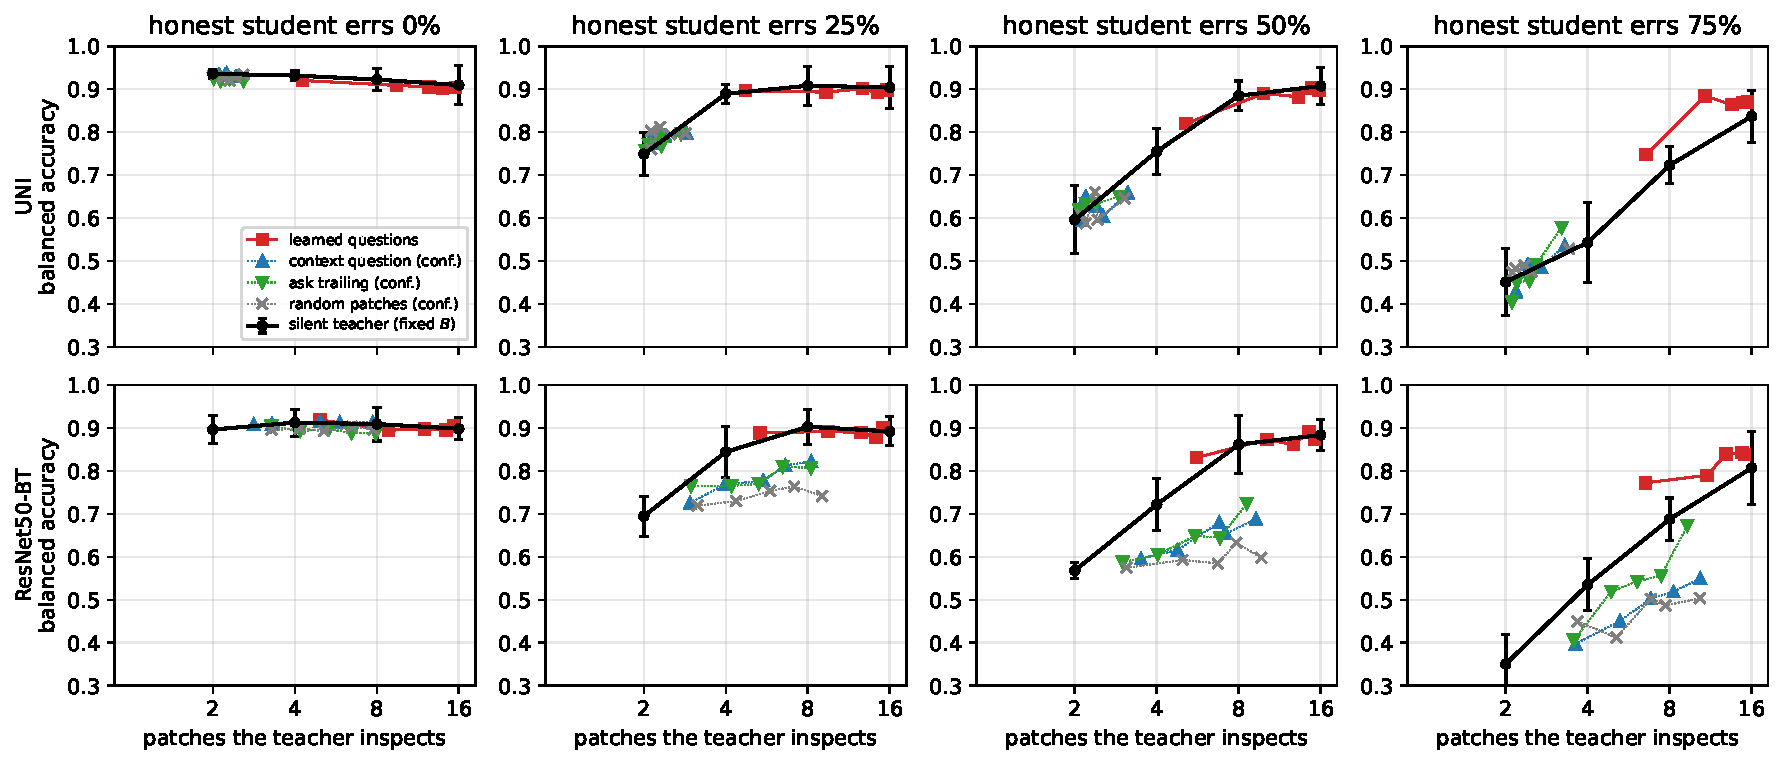
\includegraphics[width=\linewidth]{figs/fig_questions.pdf}
\caption{\textbf{Silent vs.\ questioning teacher} (CAMELYON16, 3 seeds, mean$\pm$sd for the silent teacher). Columns: the honest student picks a random patch instead of its best one with probability 0--75\%; the devil's advocate stays greedy. Black: silent teacher at fixed budget $B$. Red: learned questioning policy (per-patch cost $\lambda\in\{0,\dots,.05\}$; decides per slide when to stop and which question to ask). Blue/green/grey: confidence-triggered context question, ask-the-trailing-student, and two random patches ($\tau\in\{.7,\dots,.99\}$).}\label{fig:questions}
\end{figure*}
\paragraph{Does questioning the students help?} Fig.~\ref{fig:questions}. With competent students (left column) the answer is no: the silent teacher is already at .93 (UNI) / .91 (ResNet50) from 2--4 patches, and no question raises it. Questioning matters once the honest student is unreliable, which is the realistic case for a learned reader. Then the budget the silent teacher needs grows quickly: at 50\% honest errors it needs 8 patches to recover .89/.86 (2 patches: .60/.57). The learned questioning policy does not know the student's error rate, but spends more questions when the round is contested: on average 4.3, 4.7, 5.1 and 6.5 patches (UNI) as the honest error rate goes from 0 to 75\%. At matched average patches it matches the silent teacher with competent students and is ahead with unreliable ones (75\% errors: .75 at 6.5 patches vs.\ .67 for the silent teacher interpolated at the same budget, UNI; .77 vs .64, ResNet50), although seed variance is large ($\pm$.13). Questions triggered by the teacher's own confidence are no better than asking for two random patches, and with ResNet50 features they are worse than simply showing more student patches: the teacher is confidently wrong when the honest witness is missing (Tab.~\ref{tab:ask}). Useful questions must therefore be learned from what the round looks like (how contested it is, how attention splits between the students), not triggered by the teacher's confidence. With a fully random honest student, nothing recovers ($\le$.49): the protocol cannot create the evidence that no student presents.

\paragraph{Is it sparsity?} \begin{table}[t]\centering\small
\caption{\textbf{Fixed-judge sparsity grid} (CAMELYON16, $B{=}8$, judges trained on natural bags only; 3 seeds). Test tumor slides keep $t$ witnesses; all test slides are subsampled to $N$ patches. Cells: teaching round / random masking BA, and $p$ = probability that $B$ uniform draws contain a witness, $1-\binom{N-t}{B}/\binom{N}{B}$ (median slide).}\label{tab:sparsity}
\setlength{\tabcolsep}{2.2pt}
\begin{tabular}{@{}lcccc@{}}\toprule
$t\backslash N$ & 256 & 1024 & 4096 & full ($\sim$7.3k)\\\midrule
1 & .79/.51 {\tiny$p$.03} & .85/.50 {\tiny$p$.01} & .84/.49 {\tiny$p$.00} & .88/.50 {\tiny$p$.00}\\
4 & .93/.52 {\tiny$p$.11} & .93/.51 {\tiny$p$.03} & .95/.51 {\tiny$p$.01} & .94/.52 {\tiny$p$.01}\\
16 & .96/.67 {\tiny$p$.29} & .95/.53 {\tiny$p$.08} & .96/.50 {\tiny$p$.02} & .96/.49 {\tiny$p$.01}\\
all (27) & .97/.77 {\tiny$p$.58} & .96/.73 {\tiny$p$.44} & .96/.66 {\tiny$p$.30} & .96/.62 {\tiny$p$.23}\\\bottomrule
\end{tabular}\end{table}
The per-regime results retrain judges and change bag size; Tab.~\ref{tab:sparsity} separates witness count from bag size under fixed judges. Random masking is at chance whenever $p$ is small and rises with $p$ (.62$\to$.77 as $p$ goes .23$\to$.58), as uniform sampling predicts. The teaching round depends on the witness \emph{count} and hardly on bag size: one witness gives .79--.88, four .93--.95, sixteen .95--.96, for every $N$. Its advantage over random reading is the acquisition advantage of a reader that finds witnesses; what the protocol adds is that this advantage survives a devil's advocate, which attention top-$B$ (0.00 in every cell) and cooperative pairs do not.

\begin{figure*}[t]\centering
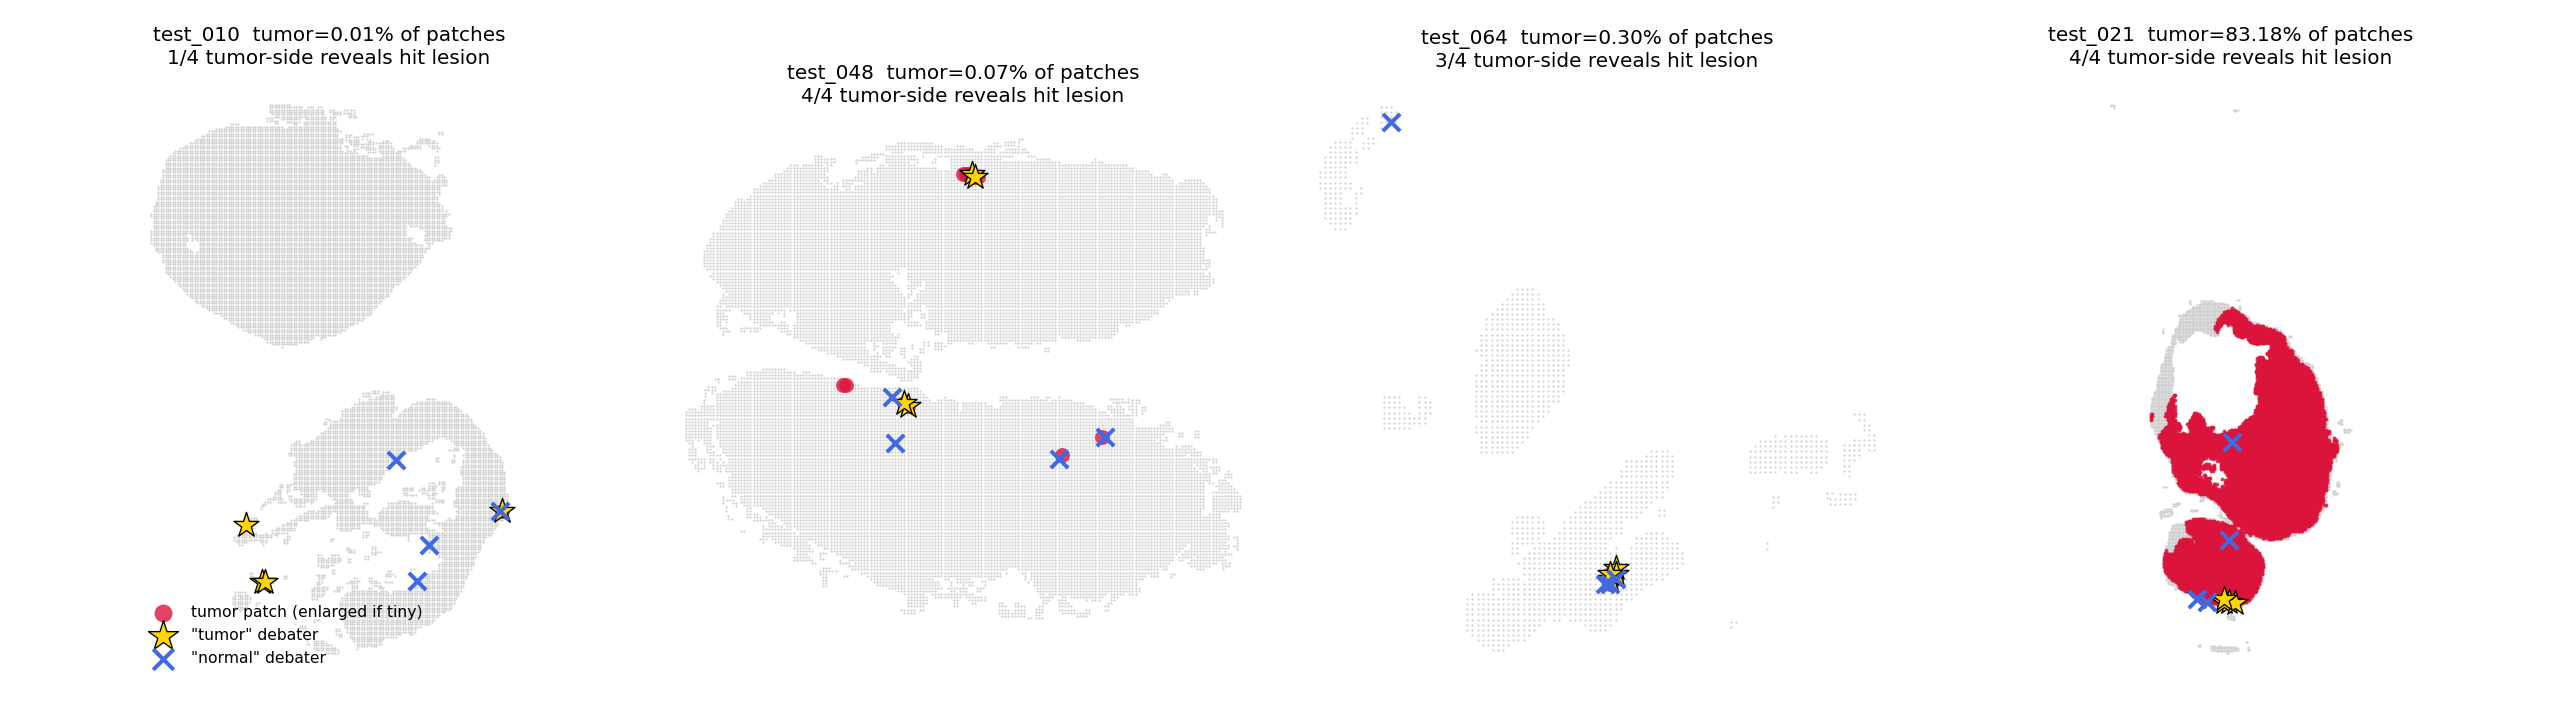
\includegraphics[width=\linewidth]{figs/fig_c16_debate.png}
\caption{\textbf{Teaching rounds on CAMELYON16 test slides} ($B{=}8$). Grey: tissue patches; red: annotated tumor (enlarged when tiny); stars: patches presented by the student arguing tumor; crosses: patches presented by the student arguing normal. Even at 0.01--0.07\% tumor, the tumor student reaches lesion patches the other student cannot hide, and the teacher needs nothing else.}\label{fig:qual}
\end{figure*}

\paragraph{Controls and failure modes.} Teachers trained from scratch on the same transcripts agree (.95--.97), and blank patches with real flags give exactly .500, so the teacher reads the patches, not the flags. The devil's advocate wins mostly by hiding (4--10\% of tumor slides at $B{=}4$--8) rather than by making normal tissue look like tumor (1--2.5\% of normal slides). A teaching round with an incompetent honest student (random picks) loses to the devil's advocate (.14--.53), and correlated omissions by both students are outside what it can repair.
\paragraph{Diffuse labels.} On BCNB, the teaching round does not beat random masking (ER .743 vs .731, PR .721 vs .736, Grade-3 .711 vs .724, $B{=}8$). Its value appears where single witnesses are decisive, which is where selection is needed most.

\paragraph{Label-free advocacy for VLMs.} \begin{table}[t]\centering\small
\caption{\textbf{One advocate per answer option} (VLM accuracy, 95\% CI; global view always shown). $n$ = number of options. Advocates and attackers choose among the same grid tiles.}\label{tab:vlmdeb}
\setlength{\tabcolsep}{2pt}
\resizebox{\linewidth}{!}{\begin{tabular}{@{}lccc@{}}\toprule
 & V* Qwen2.5 & V* Qwen3 & HR-4K Qwen2.5\\\midrule
cooperative, $n$ crops & .812 {\tiny[.75,.86]} & .911 {\tiny[.87,.95]} & .690 {\tiny[.63,.76]}\\
attacked, $n$ crops & .366 {\tiny[.29,.44]} & .335 {\tiny[.27,.40]} & .390 {\tiny[.32,.46]}\\\midrule
\textbf{advocate per option} ($n$ crops) & \textbf{.806} {\tiny[.75,.86]} & \textbf{.843} {\tiny[.79,.90]} & \textbf{.705} {\tiny[.64,.77]}\\
top-2 options advocate (2 crops) & .691 & .780 & .675\\
\ \ truth among top-2 & .859 & .901 & .815\\\bottomrule
\end{tabular}}\end{table}
For multiple-choice VQA no label is needed: every option gets a student that shows its best-supporting tile, so all but one are devil's advocates. Accuracy stays at the level of honest cooperative selection (Tab.~\ref{tab:vlmdeb}; .806/.843/.705 vs .812/.911/.690), whereas an attacker controlling the same number of crops drives it to .34--.39. Advocating only the two options most likely under the global view is weaker, because the truth is outside that pair for 10--19\% of questions: every candidate answer must be represented.

%=====================================================================
\section{Discussion and limitations}\label{sec:discussion}
\textbf{Robustness.} Greedy, look-ahead and RL-trained devil's advocates lose in our settings; this is empirical robustness to those advocates, not a worst-case guarantee. A few authentic normal patches cannot certify the \emph{absence} of a lesion: the protocol relies on a competent student who searches the whole slide for each label. \textbf{Compute.} The students still tile and read every patch, so slide I/O is not reduced; the saving is in encoder compute (15$\times$ FLOPs, 5.3$\times$ A100 time with ResNet50 students), and in what the teacher must inspect (2--16 patches of $\sim$10$^4$), which matters when the teacher is a pathologist, a large multimodal model, or an auditor. Cheaper students (lower magnification, smaller networks) are an open direction. \textbf{Scope.} The strongest results are on CAMELYON16, where single witnesses decide; on diffusely expressed BCNB labels the protocol gives no gain. We do not yet evaluate a free-text questioning teacher, or WSI agents (e.g.\ GIANT, PathFinder) in their native workflow.

\section{Conclusion}
When a judge can read only a few regions, whoever chooses them decides. Giving every answer a student, and letting a teacher that never reads the slide decide from what they present, keeps the decision near full-slide accuracy from two patches against devil's advocates that defeat every single-selector pipeline. The effective ingredient is that every label is searched for, not the interaction; and the teacher's own uncertainty cannot replace an opposing student.

{\small\bibliographystyle{ieeenat_fullname}\bibliography{refs}}
\end{document}
